%!TEX root = index.tex

\chapter{Flights Scheduling}

\label{section:scheduling}

Main goal of this thesis is to design and implement algorithm for scheduling flights arriving to airport controlled by approach controller. This chapter defines the scheduling task and presents several algorithms that provide variety of approaches to solve the task. All of the algorithms were then implemented and experiments were conducted to find the most appropriate for real-world simulation.

\section{Term Definitions}

First, let's define some terms that will be used in this chapter:

\bitem
\item \textbf{ETA} – Estimated Time of Arrival to the runway if the airplane will fly directly without delay along given STAR.
\item \textbf{EETA} – Earliest ETA among all runways ariving flight may land on. If only one runway is available $\text{EETA}=\text{ETA}$. ETA is always bigger or equal to ETA.
\item \textbf{SETA} – Scheduled ETA is the time at which the airplane is scheduled to arrive to runway. SETA is always bigger or equal to ETA.
\item \textbf{Delay} – for single runway the delay of flight arrival is defined as $\text{SETA}-\text{ETA}$, for multiple runways the delay is defined as $\text{SETA}-\text{EETA}$.
\item \textbf{Slot} – time interval assigned to arriving flight on a runway. It is defined by SETA surrounded by buffer given by accuracy of the estimate.
\eitem

\section{Problem Definition}

The approach controller's main task is to schedule aircraft flying to an airport in controlled TMA sector, given following limitations:

\bitem
\item Individual flights arrive over time and the controller becomes aware of them at the time they appear on his/hers radar screen.
\item Each flight needs to be assigned one of available runways to land on and time interval in which the assigned runway is free.
\item The runway and slot assignment must be done at the time of their appearance on the radar screen, no flights are allowed to fly in the TMA sector not knowing which runway they will land on and when.
\item The slot must be scheduled to given estimated arrival time (ETA) or later.
\item Once the runway is assigned, it must not be changed.
\item Assigned slot may be rescheduled to a later time, it may not be rescheduled earlier.
\item The slots on single runway must be spaced at least by minimum wake separation interval length. The interval length depends on weight classes of both preceding and following airplane and on their order. This means that the separation interval of \textbf{Light} airplane behind \textbf{Heavy} airplane is different (longer) than interval of \textbf{Heavy} behind \textbf{Light}.
\eitem

\subsection{Existing Algorithms Solving Similar Problems}

The task the TMA sector controller deals with is a special case of online scheduling problem. There are several algorithms providing solutions for variety of online scheduling problems \cite{scheduling}, but none were found, that would be applicable for this scheduling task. Some of the algorithms allow for jobs (corresponding to arrival slots) to wait before being assigned to one of available machines (corresponding to runways) which is not possible here. Other make the allocation of jobs to machines irreversible, in flight scheduling problem the machine (runway) selection is irreversible, but the job order on the runway is variable (with the restriction that jobs mustn't be rescheduled earlier). Some algorithms allow job preemption which is not allowed in flight scheduling. There are algorithms that allow temporal constraints between jobs, but the constraints are static, here the temporal constraints are dynamic, they only apply for jobs scheduled directly behind each other on single machine and depend on the job's order. Additionally the algorithms search for optimal solution according to single criterion, whereas in flight scheduling we look on several performance criteria and don't search for optimal result but try to find good solution by as many criteria as possible.

\subsection{Evaluation Criteria}

The criteria the TMA sector controller takes into account while scheduling approaching flights are following:

\bitem
\item \textbf{Makespan} – the length of scheduled runway plan, which is equal to the difference between SETA of last and first task on the runway. For multiple runways the makespan is defined as difference between SETA of last and first task among all runways. Makespan expresses the quality of the schedule in terms of system efficiency and airport throughput and safety, as plan with shorter makespan leaves more leeway for future arriving airplanes in case of unexpected increase in the incoming traffic.
\item \textbf{Total delay} – sum of all delays of scheduled arrivals. It expresses the schedule quality in terms of social welfare as lower total delay means lower fuel consumption and thus lower costs for airlines and lower emissions.
\item \textbf{Maximal delay} – maximal delay among all scheduled arrivals. It expresses the plan quality in terms of competitive welfare and safety as too long delay may cause the airplane to deplete it's fuel supply before landing and therefore lead to an accident. Also no airline want their flight to wait while other flights are landing and therefore more uniform delay distribution among all flights is desirable.
\item \textbf{Number of replanned slots} – total number of replanned slots during the scheduling (one slot may be replanned multiple times after additional slot allocations). It expresses the plan quality in terms of controller workload and safety as high number of changes in planned slots require the controller to update the instructions given to pilots and thus increasing his/hers workload.
\eitem

Because no existing algorithm providing desired properties was found, algorithms were designed specifically for the flight scheduling problem. The problem was divided to two parts. First, new slot is allocated on all available runways and then the resulting plans are compared and one runway is selected. This way the algorithm produces both slot and runway allocation. Algorithms for both parts of the problem are proposed in following sections but first visual representation of the runway plan is described so it can be used later to illustrate the outputs of individual algorithms.

\section{Runway Plan Visualization}

\label{section:runway-visualization}

Runway Plan Visualization module was designed to provide representation of the runway plan that is quick and easy to comprehend. The slots planned for approach are displayed horizontally with a timeline at the bottom with highlighted one and five minute marks.

Above the timeline there are rows representing individual runway plans. Headline of each runway plan is shown on the left side with the number of the runway on the top and names of every weight class in corresponding color shown below. Plans of different runways planned by the same algorithm are divided by gray dashed border. Plans of different runways planned by different algorithms are divided by solid black border.

Each slot in the plan is represented by a vertical green bar with a dark green line in it. The dark green line shows the exact time of SETA and the green bar surrounding it shows the interval of possible arrival as defined by the precision of arrival estimation. Flight ID is shown on the top, the color of the text indicates the weight class of the aircraft. Below the flight ID, gray wake turbulence intervals are shown for every weight class in the same order as in the plan headline. If the wake turbulence interval is active (there is an following airplane scheduled after the current slot), the corresponding interval is colored in the color of following airplane's weight class.

If there is a collision between the slots, active wake turbulence interval of the preceding slot and the slot itself of the following flight are shown in red color. If a slot is delayed, vertical orange line marks the time of original ETA and is connected to the delayed ETA with horizontal orange line. In multi-runway scenarios, earliest ETA among all runways (EETA) is marked by dotted orange line and is again connected with the delayed ETA with horizontal dotted line. This way the controller can distinguish which part of the delay is caused by the order of slot on the runway and which part of the delay is the runway selection responsible for.

Examples of algorithm outputs shown in this chapter are results generated by individual algorithms for scenario defined in Table \ref{tab:config-simple}. The scenario was chosen specifically to illustrate different results produced by the algorithms.

\begin{table}[h]
  \centering
\begin{tabular}{ | l | c | r | r | }
\hline
Flight id   & Weight class & Appearance on screen & Estimated arrival time \\
\hline
01          & MEDIUM       & 14:48                & 48:09 \\
02          & MEDIUM       & 17:36                & 44:23 \\
03          & JUMBO        & 19:00                & 46:11 \\
04          & JUMBO        & 19:24                & 44:11 \\
05          & MEDIUM       & 21:36                & 48:23 \\
\hline
\end{tabular}
  \caption{Configuration of the scenario illustrating different outputs generated by individual algorithms}
  \label{tab:config-simple}
\end{table}

\section{Slot Allocation on Single Runway}

\label{section:slot-selection}

This section presents several algorithms designed to allocate arrival slot on single runway. The input of the algorithm is ETA, airpane's weight class and slot size, output is the runway plan with new allocated slot.

\subsection{Algorithm 0 – Force Slot on ETA}

\begin{figure}[h]
    \centering
    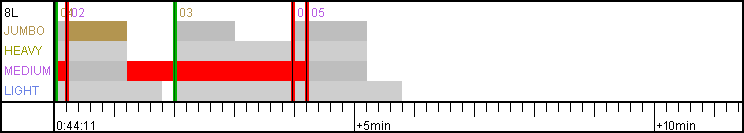
\includegraphics[width=\textwidth]{figures/rwy-in-place.png}
    \caption{Example of runway plan with colliding slots}
    \label{fig:rwy-in-place}
\end{figure}

An example of a plan generated by Algorithm 0 is shown in Figure \ref{fig:rwy-in-place}. This algorithm is the simplest of all implemented, it doesn't perform any deliberation on where to put the slot in the plan and simply places it in the time the aircraft is expected to arrive, ignoring possible collisions with other aircraft. This algorithm is not intended for actual use and serves only for comparison to other algorithms and to allow analysis of the traffic flow: it shows how many collisions there are or if the airplanes arrive to the runway periodically or in groups.

\subsection{Algorithm 1 – Keep Order of Appearance on Radar}

\begin{figure}[h]
    \centering
    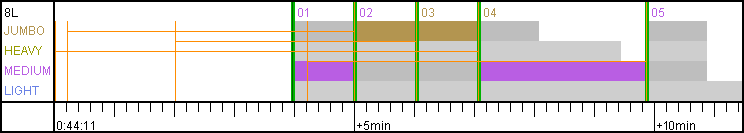
\includegraphics[width=\textwidth]{figures/rwy-end.png}
    \caption{Example of runway with slots in the order of airplane's first appearance}
    \label{fig:rwy-end}
\end{figure}

Algorithm is a simple first-come, first-served algorithm that produces valid plans with no collisions between slots. When new airplane appears on radar screen it's slot is created after all previously planned slots and not sooner than at the airplane's ETA.

Figure \ref{fig:rwy-end} shows an example of a plan generated by this algorithm. It is clearly visible that unnecessary delays can occur when the interval between the time when the airplane shows on the radar and its ETA differ from airplane to airplane. This can happen when the arrival routes have different lengths. Approach route for airplane heading directly to runway will be much shorter than for airplane arriving from opposite direction, because such airplane must first fly around the airport before landing. See Figure \ref{fig:routes} for example, the routes from south-west are significantly shorter than routes from south-east. In the example plan shown in Figure \ref{fig:rwy-end} flight \texttt{04} will arrive more than 7 minutes late because it appeared on the radar screen later than flights \texttt{01}, \texttt{02} and \texttt{03} even though its ETA is smallest.

\subsection{Algorithm 2 – Find First Empty Space in Which The Slot Fits}

\begin{figure}[h]
    \centering
    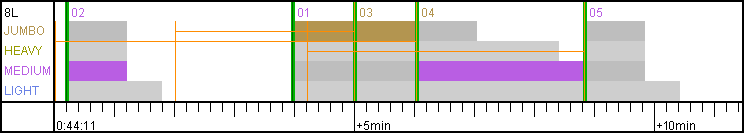
\includegraphics[width=\textwidth]{figures/rwy-fill-voids.png}
    \caption{Example of runway plan with slots fixed in place}
    \label{fig:rwy-fill-voids}
\end{figure}

Algorithm 2 creates the slot for arriving airplane in the first empty space following airplanes ETA in which the slot fits. The wake turbulence separation minima is taken into account for both preceding and following slot so no collisions between slots occur. The advantage of this this algorithm is its simplicity and the fact that the planned slots are fixed. This means that if the controller assigns a slot to airplane and clears it for approach he/she doesn't have to alter the airplane's clearance and can focus on other arriving aircraft.

An example of a plan generated by Algorithm 3 is shown in Figure \ref{fig:rwy-fill-voids}. In comparison to plan generated by previous algorithm (\ref{fig:rwy-end}) it is apparent that flight \texttt{02} can land sooner than \texttt{01} even though it entered the controlled area later. However \texttt{03} and \texttt{04} won't fit the void between \texttt{02} and \texttt{01}, and must be scheduled after. \texttt{05} would fit but arrives to the runway too late.

\subsection{Algorithms 3a, 3b – Keep Order of ETA (With Local Optimization)}

\begin{figure}[h]
    \centering
    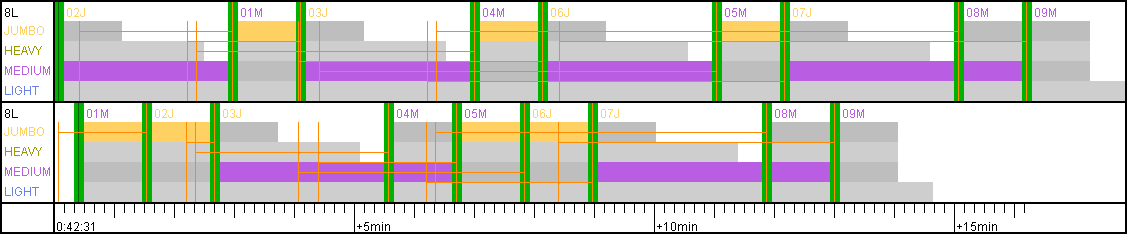
\includegraphics[width=\textwidth]{figures/rwy-eta-order.png}
    \caption{Example of runway plan that preserves the order of ETA}
    \label{fig:rwy-eta-order}
\end{figure}

Third algorithm was implemented in two variants, the first one ({\em 3a}) schedules the slots in a way that strictly preserves the order of estimated time of arrival. If the slot doesn't fit, any already planned slots following this one are delayed. If there is a continuous stream of airplanes scheduled for approach one after other and new, early arriving airplane appears on the radar screen the controller using this algorithm will squeeze the airplane in and postpone all airplanes following in the stream. This prevents a situation where the new airplane would wait for all the airplanes in the stream to land first. On the other hand the controller may need to postpone a significant number of previously planned aircraft which would take a considerable amount of time.

The second variant ({\em 3b}) is not strict with the order according to ETA. It finds the place where the new slot would fit by the ETA, but inserts it only if the delay of the following slot after the new slot is inserted is smaller than the delay of the new slot would be if it was placed after the following slot. Otherwise it tries to insert the new slot after the slot following it and so forth until the condition is met. This serves as a local optimization of the maximal delay and helps the algorithm to cope with flights with alternating weight classes.

The example plans generated by this algorithm are shown in Figure \ref{fig:rwy-eta-order}, first row contains result of variant ({\em 3a}), second row contains variant ({\em 3b}). The difference between the algorithms is visible on the order of \texttt{02} and \texttt{04}. \texttt{02} is planned first (from these two) directly on its ETA. When the \texttt{04} was inserted into the plan, variant {\em 3a} placed it before \texttt{02} because its ETA is smaller. Variant {\em 3b} with the local optimization compared the delay of \texttt{02} behind \texttt{04} with delay of \texttt{04} behind \texttt{02} and find out that the second one is smaller and therefore pushed \texttt{04} behind \texttt{02}. Before placing \texttt{04} it compared it with \texttt{03} and when delay of \texttt{03} behind \texttt{04} was smaller than the other way around it placed the slot \texttt{04} between \texttt{02} and \texttt{03}.

\subsection{Algorithms 4a, 4b, 4c – Branch And Bound}

\begin{figure}[h]
    \centering
    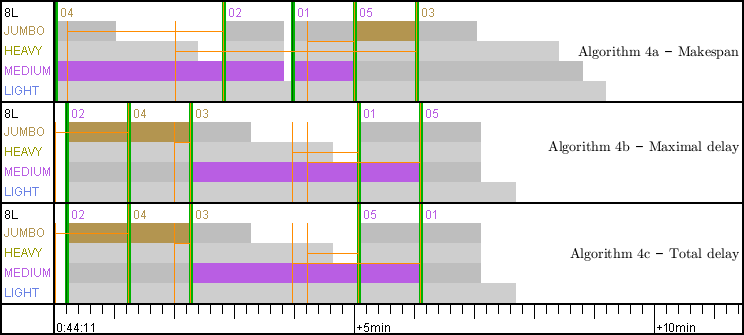
\includegraphics[width=\textwidth]{figures/rwy-bab.png}
    \caption{Comparison between the three variants of Algorithm 4}
    \label{fig:rwy-bab}
\end{figure}

Algorithm 4 is an algorithm commonly used in combinatorial optimization and is called Branch and bound. \cite{bab} The algorithm is used here in three different variants, each optimizing different criterion. Variant {\em 4a} minimizes makespan.  Variant {\em 4b} minimizes maximal delay. Variant {\em 4c} minimizes the sum of delays of all planned slots.

Figure \ref{fig:rwy-bab} shows a comparison between the three variants of Algorithm 4. It shows that the variant {\em 4a} indeed produces plan with smallest makespan but with big delays for some slots. {\em 4b} and {\em 4c} produce plans with same total delay but {\em 4b} has smaller maximal delay.

\begin{figure}[h]
    \centering
    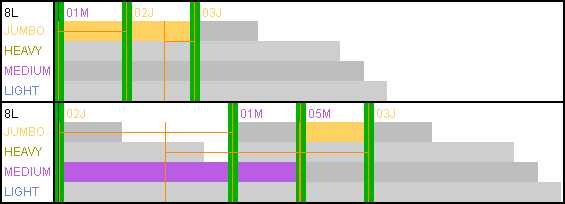
\includegraphics[width=0.7\textwidth]{figures/rwy-proof.png}
    \caption{Example of adding later slot causing changes in plan before its ETA, first row shows plan before addition of slot \texttt{D}, second row shows plan after addition}
    \label{fig:rwy-proof}
\end{figure}

There are two disadvantages of branch and bound algorithm that limit its use in real world applications.

The first one is that it doesn't keep the relative order of previously planned slots. This is caused by the fact that the algorithm is an offline algorithm and recomputes the whole plan from scratch every time new slot needs to be added. This is illustrated in Figure \ref{fig:rwy-proof} where addition of slot for flight \texttt{D} caused the order of slots for \texttt{A}, \texttt{B} and \texttt{C} to change. Changing the order of flights scheduled on a route to one runway would result in need of special behavior that would allow the airplane to leave the route, wait in a separate area until the following aircraft flies past on the route and then return back to the route. And because the complete replanning takes place every time new airplane appears on a screen it could happen that two flights would switch their place in the sequence back and fort multiple times before reaching runway.

Additionally the planned delay may decrease for any given airplane in time (see \texttt{B} in Figure~\ref{fig:rwy-proof}). But if the airplane already performed certain manoeuvre to slow it down to accommodate the delay prescribed by the previous plan, it may be impossible to speed up to reach the runway in time planned by the updated plan, even if it would be able to do so before the hold-up.

\begin{table}[h]
  \centering
\begin{tabular}{ | l || r | r | r | r | r | r | }
\hline
			& 10 slots	& 11 slots	& 12 slots	& 13 slots	& 14 slots	\\
\hline
4a – Makespan	& $< 1s$	& $3s$		& $37s$		& –			& –			\\
4b – Maximal delay	& $< 1s$	& $< 1s$	& $< 1s$	& $7s$		& $33s$		\\
4c – Total delay	& $< 1s$	& $4s$		& $45s$		& –			& –			\\
\hline
\end{tabular}
  \caption{Run times of the three variants of Branch and bound algorithm}
  \label{tab:alg5-runtime}
\end{table}

The second disadvantage of this algorithm is also linked to the need to recompute the whole plan with each slot addition and it is the computational complexity of the Branch and bound algorithm.

The algorithm enumerates possible solutions in a systematic way that ensures the optimum will be found eventually. To prevent searching through the whole state space, upper and lower bounds are used to prune the unpromising branches from the search tree. The minimal solution found so far can act as an upper bound pruning all branches with partial plans whose criterion value is already bigger or equal to the optimum. This is especially beneficial for the second variant minimizing maximal delay among all slots, because the pruning takes place early on in the search tree, eliminating many non-optimal solutions.

For optimizing makespan any empty voids in the plans can be used as a bound for the solution. This can be done if the slots are ordered according to their ETA. In such case if the ETA of the next added slot is later than the end of the previous slot and forms an empty void before it, the optimal solution lies in a tree rooted by the added slot. This is because rearranging the order of previous slots wouldn't allow the next slot to start sooner than it starts in the current partial solution. This bound cannot be used in variants 2 and 3, because rearranging previously planned slots can still improve maximal and total delay.

The sum of tasks that remain to be planned added to the length to the current partial plan can serve as an upper bound to the solution. If this value exceeds the value of the minimal solution found so far it is obvious that planning the remaining tasks cannot result into better result and current sub-tree can be pruned. This bound cannot be effectively used in this planning problem, because the size of the slots isn't constant and therefore the size of the sum depends on the order in which the slots are added to the plan. And finding the order of the slots that produces the smallest sum equals to the planning problem itself.

The previously mentioned restrictions limit the benefits of pruning and the algorithm must therefore search through a significant part of the state space which makes it slow. The Table \ref{tab:alg5-runtime} shows the runtime for rather small instances of the planning problem. The algorithm would not be useful for faster than real time simulation as is, but may serve as reference algorithm for small instances or in combination with online planning algorithm (for example for local optimization run on several neighboring slots around newly added one). 

\section{Runway Selection}

\label{section:runway-selection}

When the configuration of STARs and the airport allows the airplanes to land on one of several runways, the air traffic controller must not only decide on the order in which the airplanes land on the runway but also on which airplane lands on which runway.

The procedure for runway selection goes as follows: For every runway the arriving airplane can land on, new plan is created incorporating the slot for the incoming airplane. The plans are created using the single-runway algorithms introduced in previous section. Then all the created plans are compared using one of the criteria presented below and the optimal plan is used for the corresponding runway.

\bitem
\item First criterion used to compare runway plans is the number of slots on each runway. The plan with \textbf{less slots} is selected. This will keep the number of slots on runways balanced leading to even distribution of flights between runways.

\item Second criterion guides the airplane to the runway with the \textbf{smallest makespan} after the slot addition. This is another way of balancing the flights between the runways, this time taking into account the arrival times and not only number of slots.

\item Third criterion selects the runway with smallest \textbf{maximal delay} of slots planned on the runway. Note, that for multiple runway scheduling delay is defined as difference between SETA and EETA.

\item Fourth criterion for runway selection is \textbf{total delay} of all slots on the runway, again delay is defined as SETA minus EETA in this case. 

\item Last criterion used to compare runway plans is \textbf{SETA of the new slot}. The air traffic controller wants the airplanes to land as soon as possible and this criterion is focused on that. It compares the scheduled arrival times of the newly added slot and directs the airplane to the runway with lowest time. This way the airplane may fly to a runway which is further away if the runway is less utilized and allows for earlier landing than a runway that has the shortest route.
\eitem

All algorithms were implemented in AgentFly system and then different combinations of slot allocation and runway selection algorithms were evaluated to determine which combination is best suitable for simulating real-world scenarios.